\documentclass[prb,aps,twocolumn,showpacs,10pt]{revtex4-1}
\pdfoutput=1
\usepackage{dcolumn}% Align table columns on decimal point
\usepackage{bm}% bold math

%\usepackage{anysize}
\usepackage[colorlinks,hyperindex, urlcolor=blue, linkcolor=blue,citecolor=black, linkbordercolor={.7 .8 .8}]{hyperref}
\usepackage{graphicx}
%\usepackage{tabularx}
\usepackage{amsfonts}
\usepackage{amsmath}
\usepackage{amssymb}
\usepackage{amsbsy}
\usepackage{tikz}
\usepackage{caption}
\usepackage{subcaption}
\usepackage{nicefrac}
\usetikzlibrary{arrows,shapes,positioning}
\newenvironment{psmallmatrix}
  {\left[\begin{matrix}}
  {\end{matrix}\right]}
\usetikzlibrary{arrows,shapes,positioning}
\usetikzlibrary{decorations.markings}
  
 \usepackage{listings}
\usepackage{color}

\definecolor{dkgreen}{rgb}{0,0.6,0}
\definecolor{gray}{rgb}{0.5,0.5,0.5}
\definecolor{mauve}{rgb}{0.58,0,0.82}

\lstset{frame=tb,
  language=Java,
  aboveskip=3mm,
  belowskip=3mm,
  showstringspaces=false,
  columns=flexible,
  basicstyle={\small\ttfamily},
  numbers=none,
  numberstyle=\tiny\color{gray},
  keywordstyle=\color{blue},
  commentstyle=\color{dkgreen},
  stringstyle=\color{mauve},
  breaklines=true,
  breakatwhitespace=true,
  tabsize=3
}


\newcommand{\etal}{{\it et~al.}}

\graphicspath{{figures/}}

\begin{document}

\title {Project 3}

\author{Jane Kim}
\affiliation{Physics 480: Computational Physics}
\date{\today}


\begin{abstract}
\vspace*{5mm}
The trajectories and energies of planets in a gravitationally coupled system were calculated using two different algorithms for solving differential equations. The forward Euler method was straightforward to implement, but it did not produce stable orbits or conserve energy. The velocity Verlet method was only slightly more complicated than Euler's method, but it provided significantly better results. For time steps less than $\sim 22$ days, the velocity Verlet algorithm produced stable orbits and constant energies for systems with a few planets. The full solar system used a time step of $\sim 43.5$ s, and was only stable using the latter method. 
\end{abstract}

\maketitle

\section{Introduction}

The objective for this project was to simulate the solar system by solving for the equations of motion for each planet. Two different algorithms, the forward Euler method and the velocity Verlet method, were used to solve the system of coupled differential equations. Object orientation was essential in creating a readable, modular, and user-friendly program. \\

The coupled differential equations are derived in Section II, along with slight improvements which simplify the computations. The methods for solving the equations are discussed in Section III. The structure of the program and the implementation of the algorithms are presented in Section IV, and Section V describes the various unit tests developed for the project. The trajectories and energies of the planets for the Sun-Earth, Sun-Earth-Jupiter, and full solar systems are discussed in Section VI and plotted at the end of the report. Finally, the conclusion is written in Section VII. \\


\section{Theory}

The physics background required for this project is not very extensive, as the only force involved is gravity. To start simply, consider two celestial bodies with masses $M_1$ and $M_2$ at the locations $(x_1,y_1)$ and $(x_2,y_2)$ on the $x$-$y$ plane. We can obtain two coupled differential equations for the motion of $M_2$
\begin{equation}
\begin{split}
\frac{d^2x_2}{dt^2} &= \frac{GM_1(x_1-x_2)}{((x_1-x_2)^2+(y_1-y_2)^2)^{3/2}},\\
\frac{d^2y_2}{dt^2} &= \frac{GM_1(y_1-y_2)}{((x_1-x_2)^2+(y_1-y_2)^2)^{3/2}},
\end{split}
\end{equation}
\noindent using Newton's second law. Now add more planets with masses $M_3, M_4, \ ..., M_n$ into the system. Then to find the equations of motion for the $j^{th}$ planet, we need to sum over the interactions between $M_j$ and all the other $M_k$'s:
\begin{equation}
\begin{split}
\frac{d^2x_j}{dt^2} &= \sum_{\substack{{k = 1}\\k \neq j}}^n \frac{GM_k(x_k-x_j)}{((x_k-x_j)^2+(y_k-y_j)^2)^{3/2}},\\
\frac{d^2y_j}{dt^2} &= \sum_{\substack{{k = 1}\\k \neq j}}^n \frac{GM_k(y_k-y_j)}{((x_k-x_j)^2+(y_k-y_j)^2)^{3/2}}.
\end{split}
\end{equation}
\noindent This can easily be extended into three dimensions
\begin{equation}
\begin{split}
&\frac{d^2x_j}{dt^2} = \sum_{\substack{{k = 1}\\k \neq j}}^n \frac{GM_k(x_k-x_j)}{r_{j,k}^3},\\
&\frac{d^2y_j}{dt^2} = \sum_{\substack{{k = 1}\\k \neq j}}^n \frac{GM_k(y_k-y_j)}{r_{j,k}^3},\\
&\frac{d^2z_j}{dt^2} = \sum_{\substack{{k = 1}\\k \neq j}}^n \frac{GM_k(z_k-z_j)}{r_{j,k}^3},\\
r_{j,k} = &\sqrt{(x_k-x_j)^2+(y_k-y_j)^2+(z_k-z_j)^2},
\end{split}
\end{equation}
but we will focus on the two dimensional system for simplicity. 


Using convenient units can simplify these calculations considerably. We express distances in astronomical units (AU) and times in years (yr). For a simple Earth-Sun system, we can approximate Earth's orbit to be circular around a fixed Sun. Then the centripetal force on Earth is equal to the gravitational force due to the sun. If the Sun has mass $M_1$ and the Earth has mass $M_2$, then we have that
\begin{equation}
\frac{M_2 v_2^2}{r_{1,2}}=\frac{GM_1M_2}{r_{1,2}^2} \  \Longrightarrow \ GM_1 = v_2^2r_{1,2}.
\end{equation}
Based on our choice of units, the distance between the Sun and Earth $r_{1,2}$ is just 1 AU. The speed of Earth $v_2$ is given by
\begin{equation}
v_2 = \frac{2\pi r_{1,2}}{T} = 2\pi \  \frac{AU}{\text{yr}},
\end{equation}
so we have that
\begin{equation}
GM_1 = 4\pi^2 \ \frac{AU^3}{\text{yr}^2}.
\end{equation}
This quantity is precalculated and stored as \texttt{prefactor}.\\

Define the mass ratio $m_k = M_k/M_1$ for each $k=1,2,...,n$ celestial body in the system. Then (2) becomes
\begin{equation}
\begin{split}
\frac{d^2x_j}{dt^2} &= \sum_{\substack{{k = 1}\\k \neq j}}^n \frac{4\pi m_k(x_k-x_j)}{((x_k-x_j)^2+(y_k-y_j)^2)^{3/2}},\\
\frac{d^2y_j}{dt^2} &= \sum_{\substack{{k = 1}\\k \neq j}}^n \frac{4\pi m_k(y_k-y_j)}{((x_k-x_j)^2+(y_k-y_j)^2)^{3/2}}.
\end{split}
\end{equation}
Discretizing these equations allow us to map the orbits of all the planets in the system. 

\section{Method}
\subsection{Forward Euler}
The Euler method is a quick and simple algorithm for approximating the solution of first-order differential equations with the form $y'=f(y,t)$ and initial conditions $y(0)=y_0$. First, choose a time step $h$ and let $t_n = t_0+nh$. Then we have that
\begin{equation}
y(t_{n+1})=y(t_n+h)=y(t_n)+hy'(t_n)+O(h^2).
\end{equation}
If we substitute the differential equation and let $y_n\approx y(t_n)$ be the approximate numerical solution, we obtain
\begin{equation}
y_{n+1}\approx y_n+hf(y_n,t_n).
\end{equation}
Since our equations are second-order, we apply this method twice to $y'=f(y,t)$ and $y''=g(y',t)$ with initial conditions $y(0)=y_0$ and $y'(0)=v_{0}$.
\subsection{Velocity Verlet}
The velocity Verlet method is an algorithm for solving second-order differential equations with the form $y''(t)=f(y,t)$ with initial conditions $y(0)=y_0$ and $y'(0)=v_{0}$. Using the same notation as before, we have that
\begin{equation}
y_{n+1}\approx y_n+h=y_n+hy'_n+\frac{1}{2}h^2f(y_n,t_n).\\
\end{equation}
We can use Euler's method to then approximate $y'(t_{n+1})$ with a better guess for its derivative, namely,
\begin{equation}
y'_{n+1}\approx y'_n+\frac{1}{2}h(f(y_n,t_n)+f(y_{n+1},t_{n+1})).
\end{equation}

\section{Implementation}

A class called \texttt{CPlanet} was created to hold the name, mass ratio, and initial conditions of each planet. This class also includes member functions to change the mass ratio or the initial conditions. \\

Another class \texttt{CSolarSystem} contained a list of CPlanet objects called \texttt{planet\_list\_}. The total number of planets in the system is stored in an integer \texttt{planets\_}. Planets may be added to the system by using the following function:
\begin{lstlisting}
// solar_system.cpp
void CSolarSystem::add(CPlanet NewPlanet){

	planets_ += 1;
	planet_list_.push_back(NewPlanet);

	// add one column for each body in the solar system
	for(int i = 0; i < N_+1; ++i){

		x_[i].resize(planets_);
		y_[i].resize(planets_);
		vx_[i].resize(planets_);
		vy_[i].resize(planets_);

		if(dim_ == 3){
			z_[i].resize(planets_);
			vz_[i].resize(planets_);
		}
	}
}
\end{lstlisting}

The \texttt{CSolarSystem} member functions \texttt{solve\_euler} and \texttt{solve\_vv} use the forward Euler and velocity Verlet methods, respectively, to calculate the trajectories of all the planets during the time window $[t_0, t_f]$. 
Thus to employ these functions properly, we designate an integer \texttt{N\_} for the number of time steps between $t_0$ and $t_f$ and let the time step \texttt{h\_} be given by
\begin{equation}
h\text{\_} = \frac{t_f-t_0}{N\text{\_}}.
\end{equation}

Each point in time $t_i = t_0+i$\texttt{h\_}, with $i=0,1,2, ..., N$, was stored in a \texttt{CSolarSystem} member vector. Since the force on one planet requires the positions of all the other planets in the system, the calculations of the trajectories were stored in several matrices. The matrices \texttt{x\_} and \texttt{y\_} contain the positions in the $x-$ and $y-$ directions, while the matrices \texttt{vx\_} and \texttt{vy\_} contain the velocities. The columns in the matrices represent the planets in the system, so the matrices must be resized when new planets are added (see previous code excerpt). There are $N+1$ rows in each matrix to store the calculations for each time step. Storing the computations in this way allows for easy extraction of the distances between planets.\\

Notice that the names of the class members are always followed by an underscore. For example, the name of a planet is stored in a string \texttt{name\_}. This notation helps us keep track of the elements that can be changed by the use of a member function. The \texttt{CSolarSystem} functions \texttt{solve\_euler} and \texttt{solve\_vv} call another function named \texttt{get\_acceleration} which calculates the acceleration of the $j^{th}$ planet due to the other planets in the system during the $i^{th}$ time step.
\begin{lstlisting}
// solar_system.cpp
void CSolarSystem::get_acceleration(int i, int j, double& ax, double& ay, double& az){

	double m, r, r3;

	ax = 0.0;
	ay = 0.0;
	az = 0.0;
	for(int k = 0; k < planets_; k++){
		if(k != j) {
			m = planet_list_[k].m_;
			r = distance(i, j, k);
			r3 = r*r*r;
			ax += prefactor*m*(x_[i][k]-x_[i][j])/r3;
			ay += prefactor*m*(y_[i][k]-y_[i][j])/r3;	
			if(dim_ == 3) az += prefactor*m*(z_[i][k]-z_[i][j])/r3;	
		}
	}	
}
\end{lstlisting}
In addition, the \texttt{distance} function calculates the distance between the $j^{th}$ and $k^{th}$ planets during the $i^{th}$ time step:
\begin{lstlisting}
//solar_system.cpp
double CSolarSystem::distance(int i, int j, int k){

	double x, y, z = 0;

	x = x_[i][j]-x_[i][k];
	y = y_[i][j]-y_[i][k];
	if(dim_ == 3) z = z_[i][j]-z_[i][k];

	return sqrt(x*x+y*y+z*z);
}
\end{lstlisting}
In the Earth-Sun system, the center of mass is within the radius of the Sun so it is a fair approximation to simply keep the Sun fixed at (0,0). However, for most other situations, it is more appropriate to use the center of mass frame and let the Sun have a momentum such that the total momentum of the system is zero. Since this requires changing the initial conditions of the system, the \texttt{CSolarSystem} class has the option to "switch on" the center of mass frame. It also has the option to add a third dimension to the system.  The changes to the initial conditions are performed in the following function:
\begin{lstlisting}
//solar_system.cpp
void CSolarSystem::initialize(){

	// initial conditions of planets (including sun)
	for(int j = 0; j < planets_; j++){

		x_[0][j] = planet_list_[j].x0_[0];
		y_[0][j] = planet_list_[j].x0_[1];
		vx_[0][j] = planet_list_[j].v0_[0];
		vy_[0][j] = planet_list_[j].v0_[1];

		if(dim_ == 3){
			z_[0][j] = planet_list_[j].x0_[2];
			vz_[0][j] = planet_list_[j].v0_[2];		
		}
	}

	// shift initial positions if center-of-mass option is chosen
	// change initial velocity of sun so that total momentum = 0
	CM_[0] = 0.0;
	CM_[1] = 0.0;
	CM_[2] = 0.0;
	if(CM_frame_){

		// find center-of-mass position
		double m, xsum = 0.0, ysum = 0.0, zsum = 0.0;
		for(int j = 0; j < planets_; j++){

			m = planet_list_[j].m_;
			xsum += x_[0][j];
			ysum += y_[0][j];
			CM_[0] += m*x_[0][j];
			CM_[1] += m*y_[0][j];

			if(dim_ == 3){
				zsum += z_[0][j];
				CM_[2] += m*z_[0][j];
			}
		}
		if(xsum != 0) CM_[0] = CM_[0]/xsum;
		if(ysum != 0) CM_[1] = CM_[1]/ysum;
		if(zsum != 0) CM_[2] = CM_[2]/zsum;

		cout << "CM = (" << CM_[0] << ", " << CM_[1] << ", " << CM_[2] << ")\n" << endl;

		// shift
		for(int j = 0; j < planets_; j++){
			x_[0][j] -= CM_[0];
			y_[0][j] -= CM_[1];
			if(dim_ == 3) z_[0][j] -= CM_[2];
		}

		// zero out momentum
		double px = 0.0, py = 0.0, pz = 0.0;
		for(int j = 1; j < planets_; j++){
			m = planet_list_[j].m_;
			px += m*vx_[0][j];
			py += m*vy_[0][j];
			if(dim_ == 3) pz += m*vz_[0][j];
		}
		m = planet_list_[0].m_;
		vx_[0][0] = -px/m;
		vy_[0][0] = -py/m;
		if(dim_ == 3) vz_[0][0] = -pz/m;
	}
}
\end{lstlisting}

After the \texttt{initialize} function is called, the system is ready to solve. We can use either \texttt{solve\_euler} or \texttt{solve\_vv} to fill out the matrices \texttt{x\_}, \texttt{y\_}, \texttt{vx\_}, \texttt{vy\_} (also, \texttt{z\_} and \texttt{vz\_} if \texttt{dim\_ =3}). The forward Euler method was written as
\begin{lstlisting}
if(CM_frame_) j0 = 0;
else{
	j0 = 1;

	// fix the sun at (0,0)
	x_[i][0] = 0.0;
	y_[i][0] = 0.0;
	vx_[i][0] = 0.0;
	vy_[i][0] = 0.0;
	if(dim_ == 3){
		z_[i][0] = 0.0;
		vz_[i][0] = 0.0;
	}			
}

// calculate orbits
for(int j = j0; j < planets_; j++){

	x_[i][j] = x_[i-1][j] + h_*vx_[i-1][j];
	y_[i][j] = y_[i-1][j] + h_*vy_[i-1][j];
	if(dim_ == 3) z_[i][j] = z_[i-1][j] + h_*vz_[i-1][j];
	get_acceleration(i-1, j, a[0], a[1], a[2]);
	vx_[i][j] = vx_[i-1][j] + h_*a[0];
	vy_[i][j] = vy_[i-1][j] + h_*a[1];
	if(dim_ == 3) vz_[i][j] = vz_[i-1][j] + h_*a[2];
}
\end{lstlisting}
to account for the options for a third dimension and the center of mass frame. The velocity Verlet method, on the other hand, uses the same \texttt{j0} as above, but the loop to calculate the orbits is
\begin{lstlisting}
// calculate orbits
for(int j = j0; j < planets_; j++){

	get_acceleration(i-1, j, a1[0], a1[1], a1[2]);
	x_[i][j] = x_[i-1][j] + h_*vx_[i-1][j] + 0.5*h_*h_*a1[0];
	y_[i][j] = y_[i-1][j] + h_*vy_[i-1][j] + 0.5*h_*h_*a1[1];
	if(dim_ == 3) z_[i][j] = z_[i-1][j] + h_*vz_[i-1][j] + 0.5*h_*h_*a1[2];

	get_acceleration(i, j, a2[0], a2[1], a2[2]);
	vx_[i][j] = vx_[i-1][j] + 0.5*h_*(a1[0]+a2[0]);
	vy_[i][j] = vy_[i-1][j] + 0.5*h_*(a1[1]+a2[1]);
	if(dim_ == 3) vz_[i][j] = vz_[i-1][j] + 0.5*h_*(a1[2]+a2[2]);
}	
\end{lstlisting}


Then the trajectories are written to file using \texttt{write\_orbits}. In this function, the number of points that are printed is limited so that the files for the full solar system are managable to plot. \\


Since there is no external torque acting on the system the angular momentum of each planet should be conserved. The angular momentum of the $j^{th}$ planet at the $i^{th}$ time step is calculated in
\begin{lstlisting}
//solar_system.cpp
void CSolarSystem::get_angmomentum(int i, int j, double& L){

	double M, v, r;

	M = planet_list_[j].m_;
	v = velocity(i, j);
	r = distance(i, j, 0);

	L = M*v*r;
}
\end{lstlisting}
Likewise, the energy must also stay conserved because the system is isolated. The energy of the $j^{th}$ planet at the $i^{th}$ time step is given by
\begin{lstlisting}
//solar_system.cpp
void CSolarSystem::get_energy(int i, int j, double& E){

	double M, m, v, r;

	// kinetic energy
	M = planet_list_[j].m_;
	v = velocity(i,j);
	E = 0.5*M*v*v;

	// potential energy
	for(int k = 0; k < planets_; k++){
		if(k != j){
			m = planet_list_[k].m_;
			r = distance(i, j, k);
			E += -prefactor*M*m/r;
		}
	}
}
\end{lstlisting}


\section{Tests}

Four test cases were generated to examine the properties of the program. In all four cases, the velocity Verlet method was used to solve the simple Sun-Earth system. Earth was initially placed at $(x,y)=(1 AU, 0)$ and given an initial velocity of $2\pi \frac{AU}{yr}$ in the positive $y$-direction. 
 
\subsection{Conservation of Energy}
To test the conservation of energy, we first chose a small enough step size \texttt{h\_}$=10^{-4} \text{yr} = 52.6$ min so that our calculations were very stable. The initial energy of the system was calculated using \texttt{get\_energy} and compared to the energy of Earth at every 100 time steps during one full orbit. 

\subsection{Conservation of Angular Momentum}
The conservation of angular momentum was tested in a similar way. The function \texttt{get\_angmomentum} returned the initial angular momentum of earth, which was then compared to the angular momentum at later times. 

\subsection{Stability of Earth's Orbit}
To check that Earth's orbit remain stable over the course of 1000 years, we required that the distance between the Sun and the Earth was 1 AU at serveral different times. The step sized used in this case was the same as before.

\subsection{Escape Velocity of Earth}
If Earth's initial velocity is too large, it can fall out of the Sun's orbit. The theoretical escape velocity of Earth, or the minimum speed needed to escape the Sun's orbit, is given by 
\begin{equation}
v_e = \sqrt{\frac{2GM_1}{r_{1,2}}} = \sqrt{2(4\pi^2)} = \sqrt{2}2\pi \approx 8.886\  \frac{AU}{yr}.
\end{equation}
The escape velocity was found numerically by employing a variation of the bisection algorithm. We first defined the window for the escape velocity as [min,max]=[$2\pi$,$3\pi$] then used the following algorithm to narrow the window around the escape velocity
\begin{lstlisting}
while(max-min > 1.0E-5){

	v0 = 0.5*(min+max);
	CPlanet sun("Sun", 1.0, 0.0, 0.0, 0.0, 0.0, 0.0, 0.0);
	CPlanet earth("Earth", 3.0E-6, 1.0, 0.0, 0.0, 0.0, v0, 0.0);
	CSolarSystem test(N, 2, 0, 1, false);
	test.add(sun);
	test.add(earth);
	test.initialize();
	test.solve_vv();
	test.get_energy(N, 1, E);
	if(E < 0) min = v0;
	if(E > 0) max = v0;
}
\end{lstlisting}
A time step of \texttt{h\_}$=10^{-5} \text{yr}=5.26$ provided enough accuracy to correctly find the escape velocity up to 5 places after the decimal point. 

\section{Results}
All four tests, consisting of 10204 assertions, were passed. We were also interested in comparing the two algorithms for solving differential equations and producing stable systems. In the Sun-Earth binary system, Euler's method yielded noticable increases in the radius of Earth's orbit over 50 years for all time steps used (see FIG. 1). One can extrapolate that even with a step size as small as \texttt{h\_}$=2.5\cdot10^{-6}$ yr $\approx$ 1.31 s, Earth would eventually spiral out of orbit. Thus it appears to be difficult for the forward Euler method to produce a stable system. \\

Alternatively, the velocity Verlet method produced stable orbits for all time steps less than \texttt{h\_}$=2.5\cdot10^{-3}$ yr $\approx$ 21.9 days. This is a significant improvement from the previous algorithm, and it is particularly apparent in the case where \texttt{h\_}$=0.25$ yr. With the Euler method, we would expect that using a time step this large would cause Earth to immediately leave the orbit of the Sun. But the velocity Verlet method corrects this behavior surprisingly quickly, as shown in FIG. 2. The orbits for the remaining time steps appear to coincide, but the energy plot reveals that Earth's energy is only constant for time steps equal to or less than 21.9 days.\\

Adding Jupiter into this system creates a trinary system. The orbits and energies of both planets are plotted in FIG. 3 and 4. Euler's method, again, failed to generate orbits that withstood the test of time. However, the scale of the energy plot makes the energies for \texttt{h\_}$=2.5\cdot10^{-6}$ yr $\approx$ 1.31 s appear constant. The velocity Verlet method created circular orbits for both planets for nearly all the time steps tested. Notice that the energies using the Euler method consistently increase over time, whereas the energies using the velocity Verlet method eventually levels off, even for large time steps. Also, notice the difference in Earth's orbit between FIG. 2 (a) and FIG. 4 (a). For the case where \texttt{h\_}$=0.25$ yr, the presence of Jupiter caused Earth to fall out of orbit immediately. 

Lastly, we created a model of the entire solar system (including Pluto) using initial conditions provided by the Jet Propulsion Laboratory's HORIZON system. For this case, we included the third dimension in the calculations and worked in the center of mass frame. A time step of \texttt{h\_} $\approx 43.5$ s was used for both methods.  Planets with smaller orbital radii orbit the Sun many times before Pluto completes one orbit. Thus the instability of Mercury, Venus, and Earth using Euler's method (FIG. 5) suggests the entire solar system is also unstable. Fortunately, the velocity Verlet method does, in fact, produce a stable solar system (FIG. 6).\\

\section{Conclusion}

Both algorithms are derived by neglecting certain higher order terms in the Taylor expansion of the solution to a differential equation. The forward Euler method is simple and intuitive to implement, but it does not conserve energy as we hope for an isolated system. Neither does it produce reliable orbits that remain stable over hundreds of years. The velocity Verlet method, on the other hand, does conserve energy and is arguably just as simple to implement. Hence the latter method is clearly superior.

\begin{figure*}
\centering
\begin{subfigure}{.5\textwidth}
  \centering
  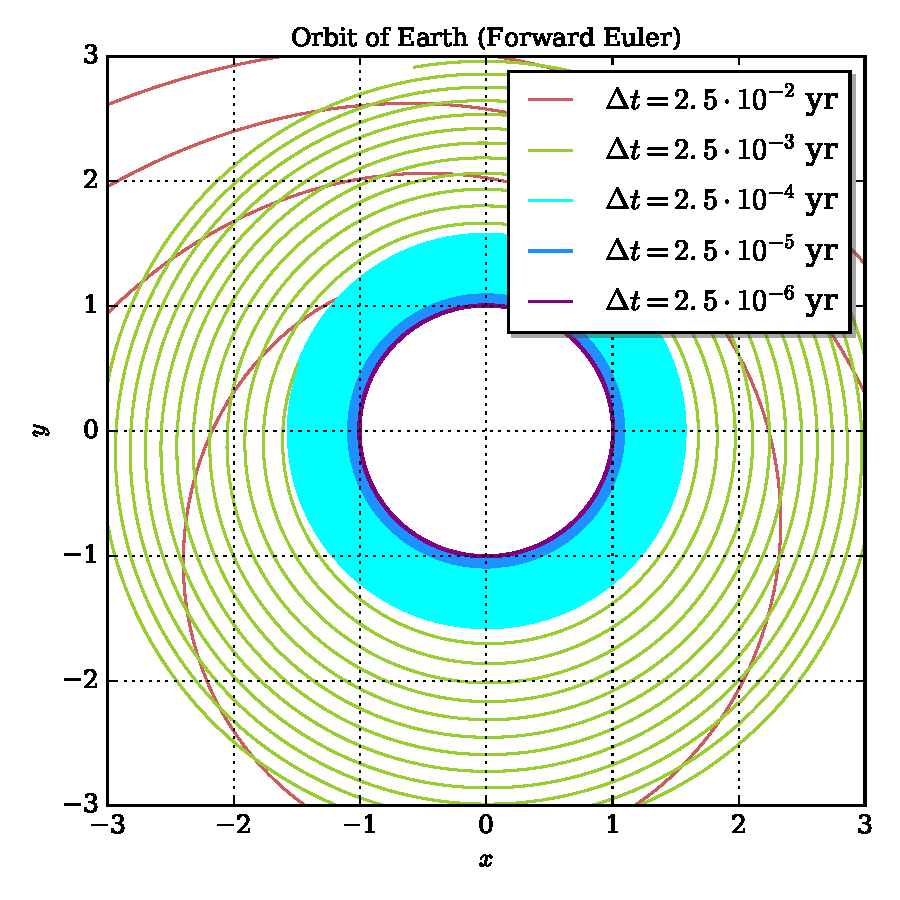
\includegraphics[width=\linewidth]{binary_fixed_euler_orbit.pdf}
  \caption{\vspace*{1mm}}
  \label{fig:sub1}
\end{subfigure}%
\begin{subfigure}{.5\textwidth}
  \centering
  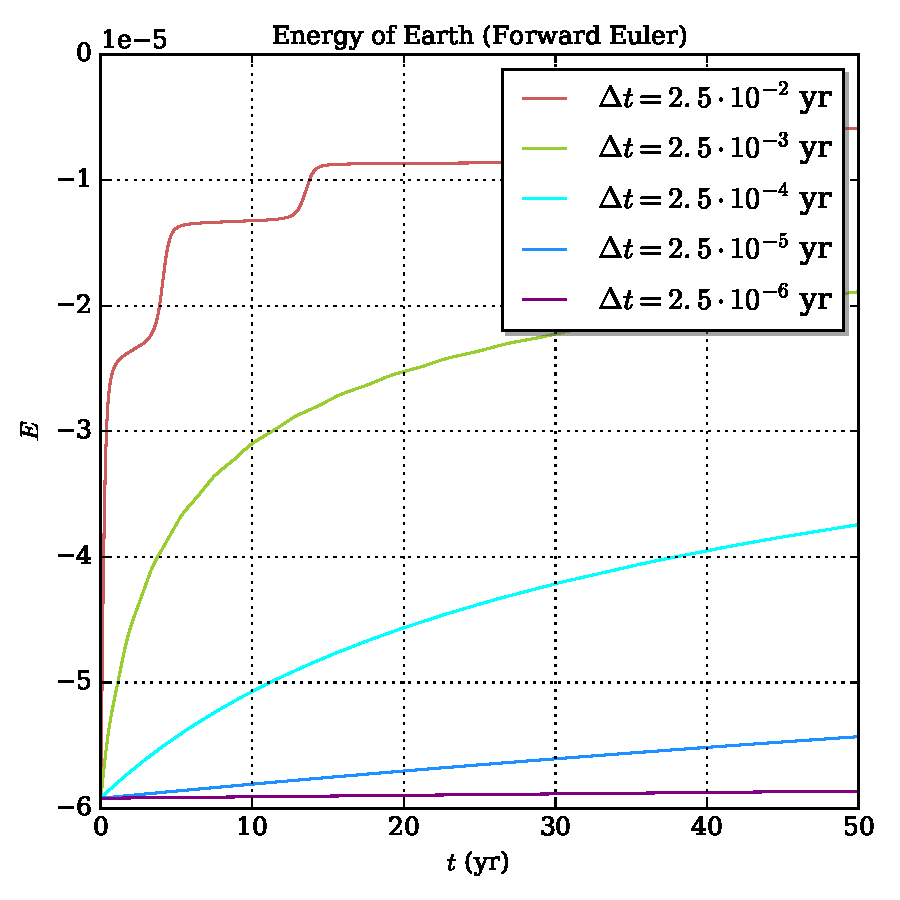
\includegraphics[width=\linewidth]{binary_fixed_euler_energy.pdf}
  \caption{\vspace*{1mm}}
  \label{fig:sub2}
\end{subfigure}
\caption{The trajectory (a) and energy (b) of Earth in the Sun-Earth binary system for several different time steps using the forward Euler method. None of the cases tested produced constant energy values.}
\label{fig:test}
\end{figure*}
\begin{figure*}
\centering
\begin{subfigure}{.5\textwidth}
  \centering
  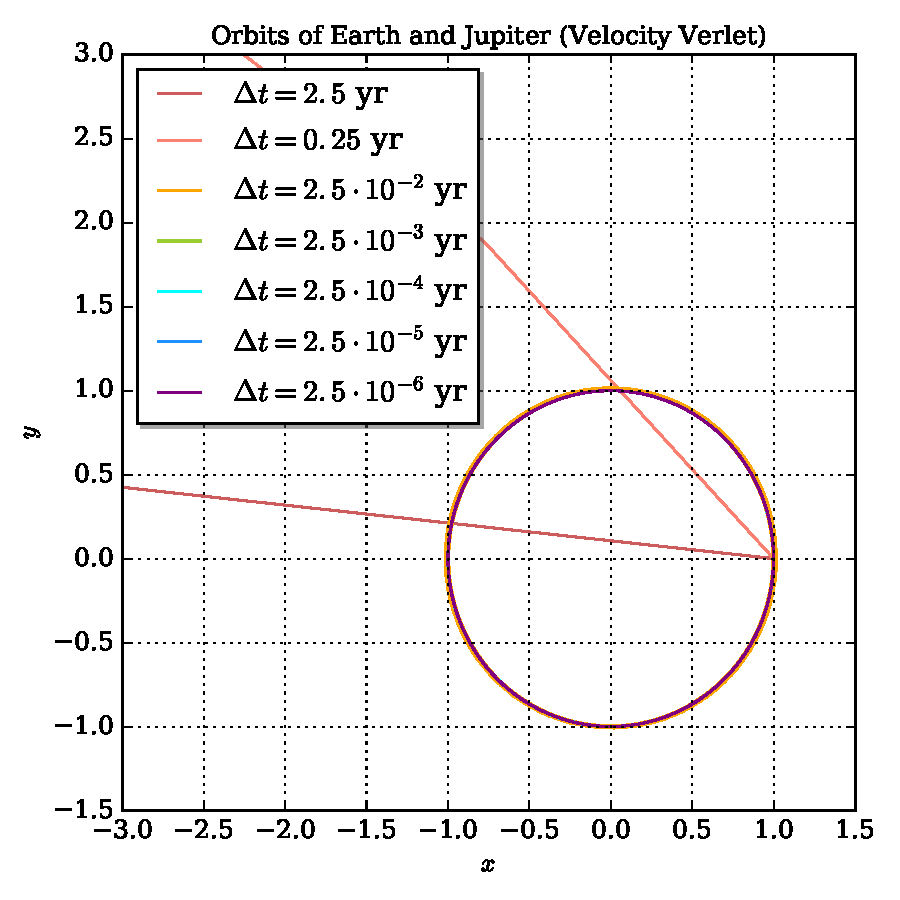
\includegraphics[width=\linewidth]{binary_fixed_vv_orbit.pdf}
  \caption{\vspace*{1mm}}
  \label{fig:sub1}
\end{subfigure}%
\begin{subfigure}{.5\textwidth}
  \centering
  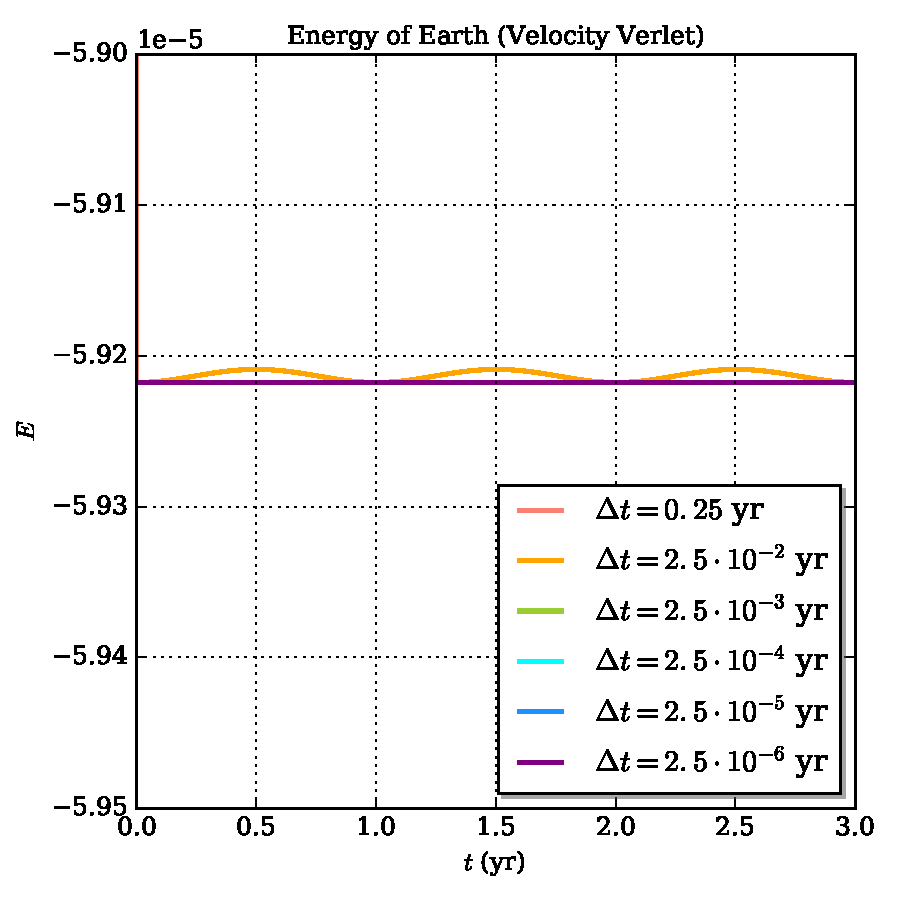
\includegraphics[width=\linewidth]{binary_fixed_vv_energy.pdf}
  \caption{\vspace*{1mm}}
  \label{fig:sub2}
\end{subfigure}
\caption{The trajectory (a) and energy (b) of Earth in the Sun-Earth binary system for several different time steps using the velocity Verlet method. Four of the six time steps produced constant energy values, all of which were also used to test the forward Euler method. }
\label{fig:test}
\end{figure*}
\begin{figure*}
\centering
\begin{subfigure}{.5\textwidth}
  \centering
  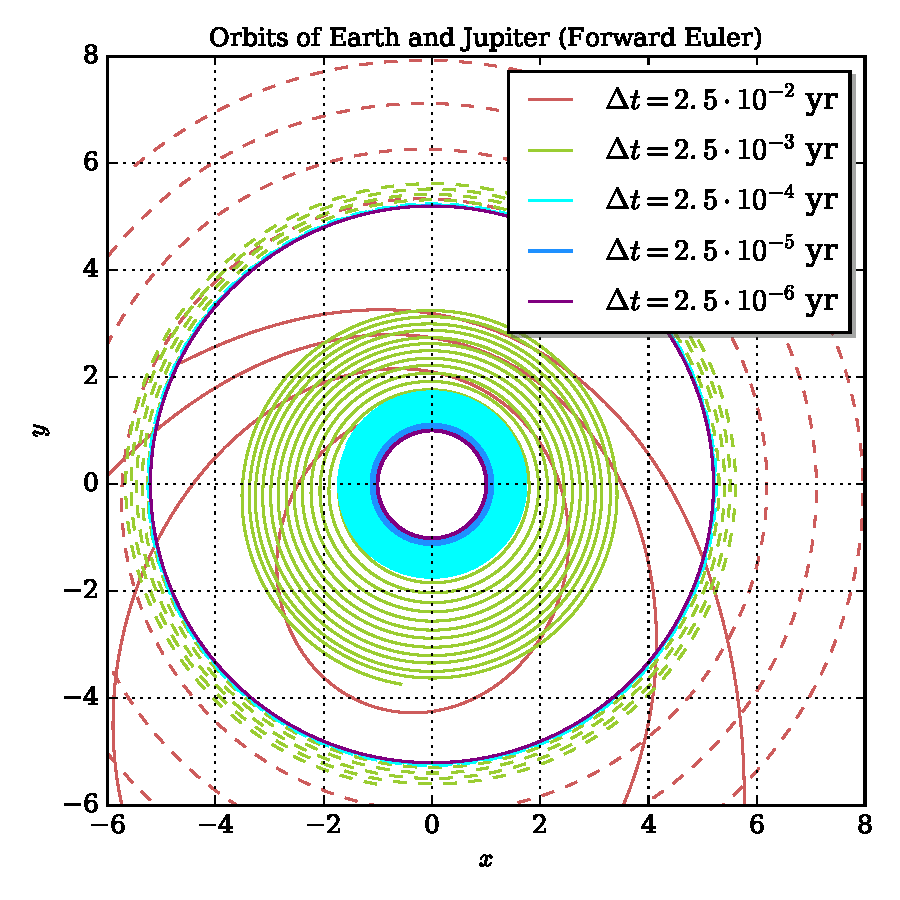
\includegraphics[width=\linewidth]{trinary_fixed_euler_orbit.pdf}
  \label{fig:sub1}
\end{subfigure}%
\begin{subfigure}{.5\textwidth}
  \centering
  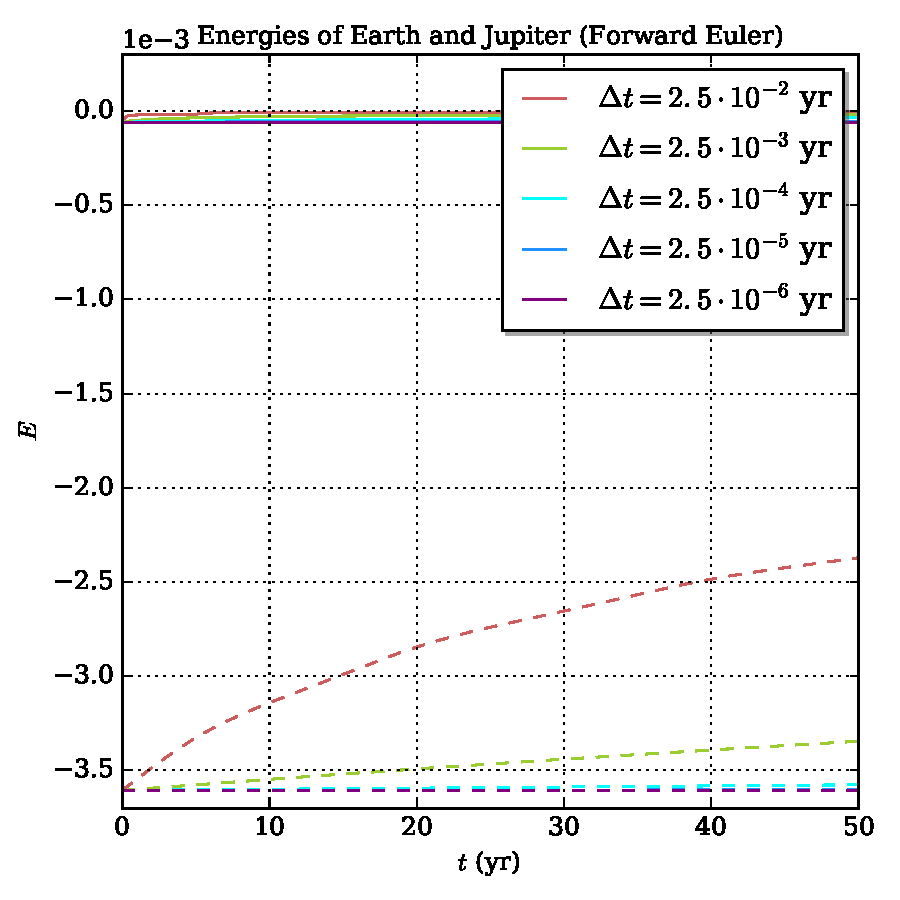
\includegraphics[width=\linewidth]{trinary_fixed_euler_energy.pdf}
  \label{fig:sub2}
\end{subfigure}
\caption{The orbits (a) and energies (b) of both Earth and Jupiter in the Sun-Earth-Jupiter trinary system using the forward Euler method. Earth is represented by the solid lines, while Jupiter is represented by the dashed lines.}
\label{fig:test}
\end{figure*}
\begin{figure*}
\centering
\begin{subfigure}{.5\textwidth}
  \centering
  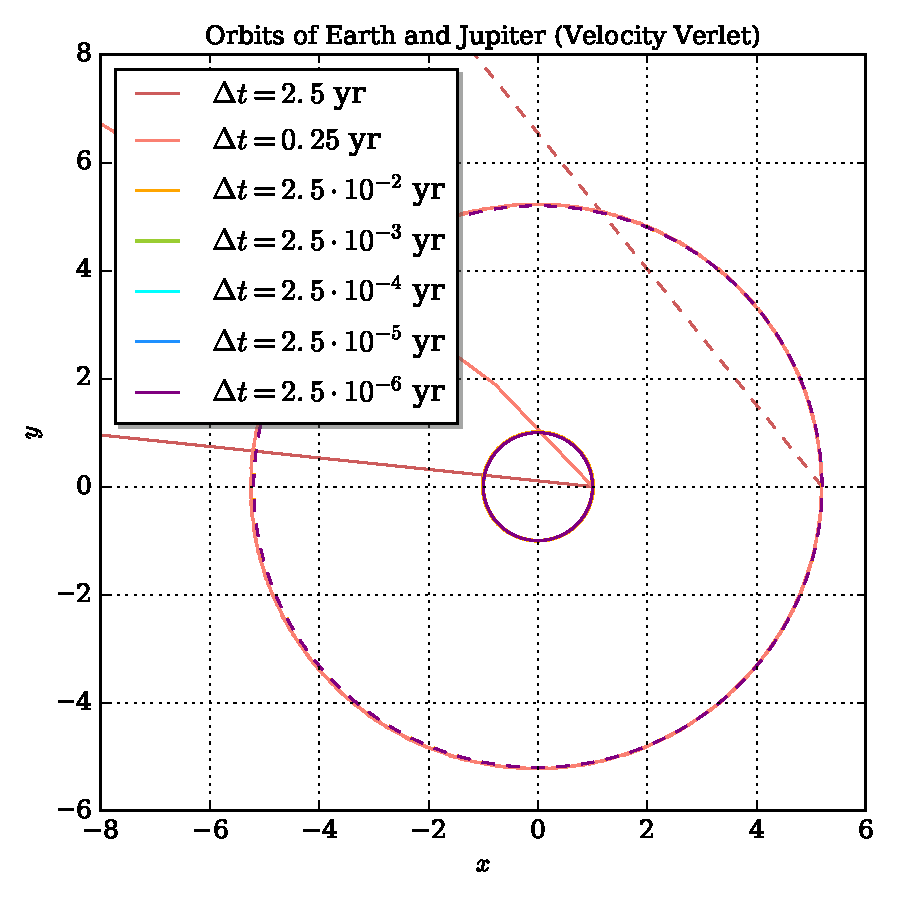
\includegraphics[width=\linewidth]{trinary_fixed_vv_orbit.pdf}
  \label{fig:sub1}
\end{subfigure}%
\begin{subfigure}{.5\textwidth}
  \centering
  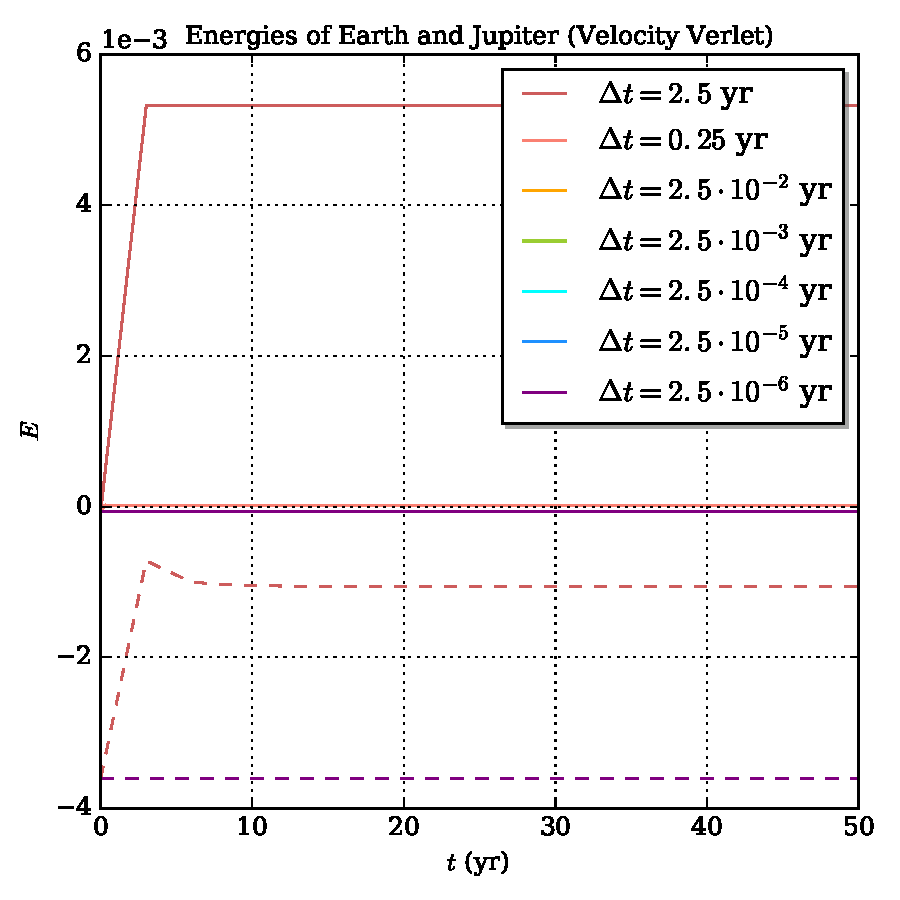
\includegraphics[width=\linewidth]{trinary_fixed_vv_energy.pdf}
  \label{fig:sub2}
\end{subfigure}
\caption{The orbits (a) and energies (b) of both Earth and Jupiter in the Sun-Earth-Jupiter trinary system using the velocity Verlet method. Earth is represented by the solid lines, while Jupiter is represented by the dashed lines.}
\label{fig:test}
\end{figure*}

\begin{center}
\begin{figure*}
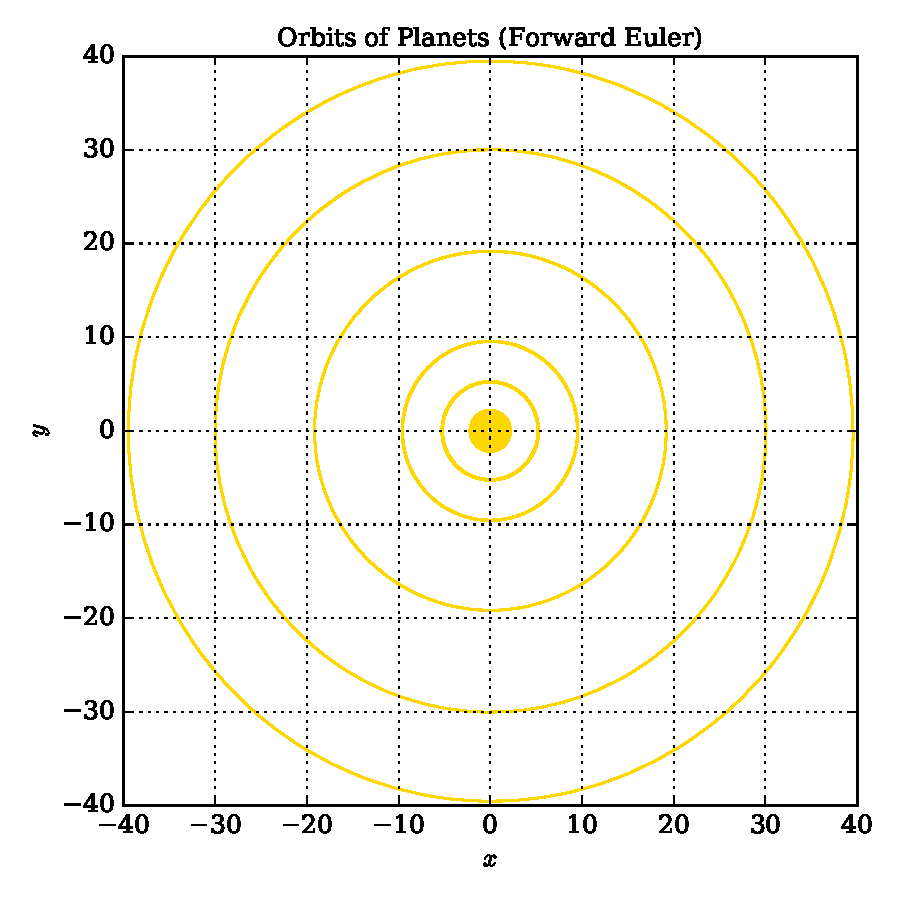
\includegraphics[scale=0.7]{solar_system_euler_orbit.pdf}
\caption{The trajectories of the full solar system using the forward Euler method.}
\end{figure*}
\end{center}
\begin{center}
\begin{figure*}
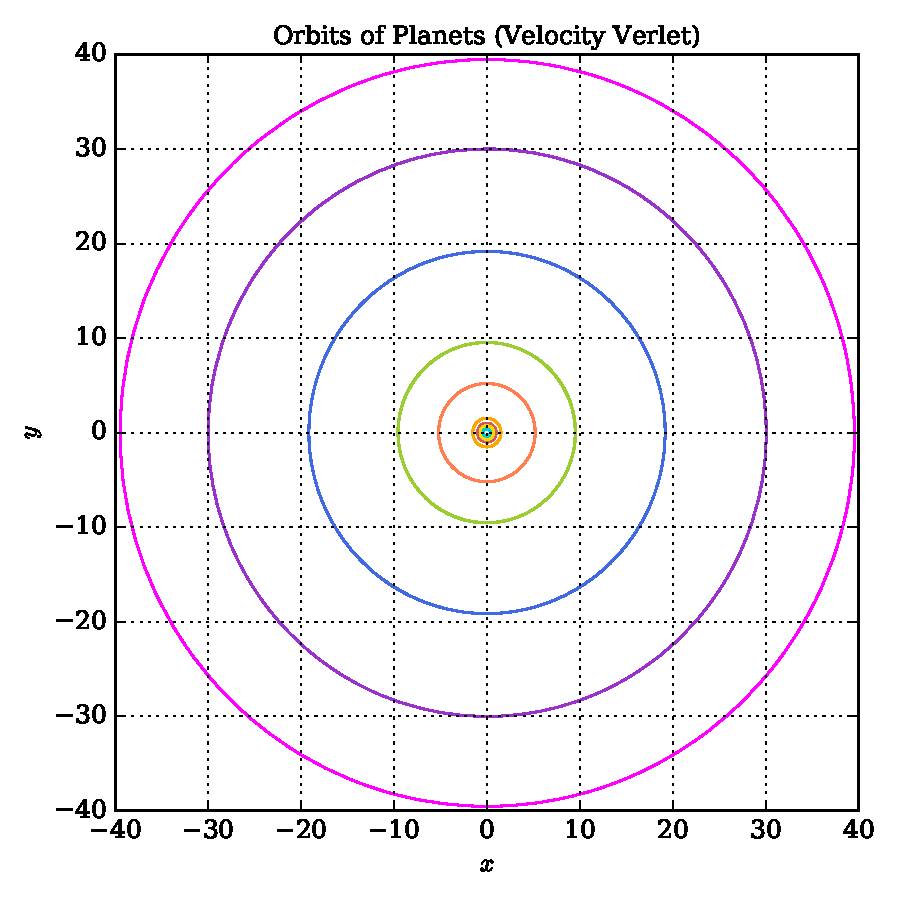
\includegraphics[scale=0.7]{solar_system_vv_orbit.pdf}
\caption{The trajectories of the full solar system using the velocity Verlet method.}
\end{figure*}
\end{center}


\begin{references}
\bibitem{notes} M. Hjorth-Jensen. "Computation Physics, Lecture Notes Fall 2015". University of Oslo. August 2015.
\bibitem{nasa} Jet Propulsion Laboratory. "Solar System Dynamics". NASA. https://ssd.jpl.nasa.gov/horizons.cgi\#top.
\end{references}

\end{document}
